\section{Logarithmusfunktionen – Die Welt des 'Zurückrechnens'}
\label{sec:logarithmusfunktionen_intro}

\begin{aufgabenumgebung}{Rechnen mit Logarithmen}
\begin{enumerate}
    \item Vereinfache die folgenden Terme so weit wie möglich (alle Variablen seien positiv):
        \begin{itemize}
            \item $\ln(x^3) + \ln(x^2)$
            \item $\ln(a^5) - \ln(a^2)$
            \item $2\ln(u) - 3\ln(v)$
            \item $\frac{1}{2}\ln(16x^4)$
        \end{itemize}
    \item Löse die folgenden Exponentialgleichungen nach $x$. Gib das Ergebnis sowohl exakt als auch als Dezimalzahl (auf 3 Nachkommastellen gerundet) an.
        \begin{itemize}
            \item $e^x = 20$
            \item $2e^{3x} = 18$
            \item $e^{-0.5x+1} = 5$
            \item $100 \cdot (0.7)^x = 10$ (Tipp: Erst isolieren, dann logarithmieren. Du kannst hier $\ln$ verwenden, obwohl die Basis $0.7$ ist.)
        \end{itemize}
\end{enumerate}
\end{aufgabenumgebung}




\begin{loesungsumgebung}[loes:rechnen-mit-logarithmen]{Rechnen mit Logarithmen}

\begin{enumerate}[label=(\alph*)]
    \item \textbf{Vereinfache die folgenden Terme so weit wie möglich (alle Variablen seien positiv):}
    \begin{itemize}
        \item $\mathbf{\ln(x^3) + \ln(x^2)}$
        $$ \ln(x^3) + \ln(x^2) = \ln(x^3 \cdot x^2) = \ln(x^{3+2}) = \ln(x^5) = \mathbf{5\ln(x)} $$
        Oder alternativ: $3\ln(x) + 2\ln(x) = (3+2)\ln(x) = 5\ln(x)$.

        \item $\mathbf{\ln(a^5) - \ln(a^2)}$
        $$ \ln(a^5) - \ln(a^2) = \ln\left(\frac{a^5}{a^2}\right) = \ln(a^{5-2}) = \ln(a^3) = \mathbf{3\ln(a)} $$
        Oder alternativ: $5\ln(a) - 2\ln(a) = (5-2)\ln(a) = 3\ln(a)$.

        \item $\mathbf{2\ln(u) - 3\ln(v)}$
        $$ 2\ln(u) - 3\ln(v) = \ln(u^2) - \ln(v^3) = \mathbf{\ln\left(\frac{u^2}{v^3}\right)} $$

        \item $\mathbf{\frac{1}{2}\ln(16x^4)}$
        \begin{align*} \frac{1}{2}\ln(16x^4) &= \frac{1}{2}(\ln(16) + \ln(x^4)) \\ &= \frac{1}{2}(\ln(2^4) + 4\ln(x)) \\ &= \frac{1}{2}(4\ln(2) + 4\ln(x)) \\ &= \mathbf{2\ln(2) + 2\ln(x)} \quad (\text{oder } 2(\ln(2) + \ln(x)) \text{ oder } \ln(4x^2)) \end{align*}
        Da $x>0$, ist $\ln(4x^2) = \ln(4) + \ln(x^2) = 2\ln 2 + 2\ln x$.
    \end{itemize}

    \item \textbf{Löse die folgenden Exponentialgleichungen nach $x$. Gib das Ergebnis sowohl exakt als auch als Dezimalzahl (auf 3 Nachkommastellen gerundet) an.}
    \begin{itemize}
        \item $\mathbf{e^x = 20}$
        $$
        \begin{array}{r c l c l}
        \umformung{e^x}{20}{\ln(\ldots)}{}
        \umformung{x}{\ln(20)}{}{}
        \end{array}
        $$
        Exakte Lösung: $x = \ln(20)$.
        Dezimalzahl: $x \approx \mathbf{2.996}$.

        \item $\mathbf{2e^{3x} = 18}$
        $$
        \begin{array}{r c l c l}
        \umformung{2e^{3x}}{18}{\div}{2}
        \umformung{e^{3x}}{9}{\ln(\ldots)}{}
        \umformung{3x}{\ln(9)}{\div}{3}
        \umformungend{x}{\frac{\ln(9)}{3}}
        \end{array}
        $$
        Exakte Lösung: $x = \frac{\ln(9)}{3} = \frac{\ln(3^2)}{3} = \frac{2\ln(3)}{3}$.
        Dezimalzahl: $x \approx \frac{2 \cdot 1.098612}{3} \approx \frac{2.197224}{3} \approx \mathbf{0.732}$.

        \item $\mathbf{e^{-0.5x+1} = 5}$
        $$
        \begin{array}{r c l c l}
        \umformung{e^{-0.5x+1}}{5}{\ln(\ldots)}{}
        \umformung{-0.5x+1}{\ln(5)}{-}{1}
        \umformung{-0.5x}{\ln(5)-1}{\div}{(-0.5)}
        \umformungend{x}{\frac{\ln(5)-1}{-0.5}}
        \end{array}
        $$
        Exakte Lösung: $x = \frac{\ln(5)-1}{-0.5} = -2(\ln(5)-1) = 2(1-\ln(5))$.
        Dezimalzahl: $x \approx 2(1-1.609438) = 2(-0.609438) \approx \mathbf{-1.219}$.

        \item $\mathbf{100 \cdot (0.7)^x = 10}$
        $$
        \begin{array}{r c l c l}
        \umformung{100 \cdot (0.7)^x}{10}{\div}{100}
        \umformung{(0.7)^x}{0.1}{\ln(\ldots)}{}
        \umformung{x \ln(0.7)}{\ln(0.1)}{\div}{\ln(0.7)}
        \umformungend{x}{\frac{\ln(0.1)}{\ln(0.7)}}
        \end{array}
        $$
        Exakte Lösung: $x = \frac{\ln(0.1)}{\ln(0.7)}$.
        Dezimalzahl: $x \approx \frac{-2.302585}{-0.356675} \approx \mathbf{6.456}$.
    \end{itemize}
\end{enumerate}

\end{loesungsumgebung}



\begin{aufgabenumgebung}{Ableiten und Integrieren mit \texorpdfstring{$\ln(x)$}{ln(x)}}
\begin{enumerate}
    \item Bilde die erste Ableitung der folgenden Funktionen:
        \begin{itemize}
            \item $f_1(x) = -2\ln(x) + e^x$
            \item $f_2(x) = x^3 \ln(x)$ (Produktregel!)
            \item $f_3(x) = \frac{\ln(x)}{x}$ (Quotientenregel!)
        \end{itemize}
    \item Bestimme die Menge aller Stammfunktionen:
        \begin{itemize}
            \item $g_1(x) = \frac{3}{x} - 2x + 1$
            \item $g_2(x) = \frac{x^2+x-1}{x}$ (Tipp: Den Bruch zuerst aufteilen!)
        \end{itemize}
\end{enumerate}
\end{aufgabenumgebung}



\begin{loesungsumgebung}[loes:ableiten-integrieren-lnx]{Ableiten und Integrieren mit \texorpdfstring{$\ln(x)$}{ln(x)}}

\begin{enumerate}[label=(\alph*)]
    \item \textbf{Bilde die erste Ableitung der folgenden Funktionen:}
    Der Definitionsbereich für Funktionen mit $\ln(x)$ ist $x>0$.
    \begin{itemize}
        \item \textbf{$f_1(x) = -2\ln(x) + e^x$} \\
        Definitionsbereich: $x>0$.
        $$ f_1'(x) = \frac{d}{dx}(-2\ln(x) + e^x) = -2 \cdot \frac{1}{x} + e^x = \mathbf{-\frac{2}{x} + e^x} $$

        \item \textbf{$f_2(x) = x^3 \ln(x)$} (Produktregel!) \\
        Definitionsbereich: $x>0$.
        Sei $u(x) = x^3 \Rightarrow u'(x) = 3x^2$. \\
        Sei $v(x) = \ln(x) \Rightarrow v'(x) = \frac{1}{x}$.
        \begin{align*}
        f_2'(x) &= u'(x)v(x) + u(x)v'(x) \\
                &= 3x^2 \cdot \ln(x) + x^3 \cdot \frac{1}{x} \\
                &= 3x^2 \ln(x) + x^2 \\
                &= \mathbf{x^2(3\ln(x) + 1)}
        \end{align*}

        \item \textbf{$f_3(x) = \frac{\ln(x)}{x}$} (Quotientenregel!) \\
        Definitionsbereich: $x>0$.
        Sei $u(x) = \ln(x) \Rightarrow u'(x) = \frac{1}{x}$. \\
        Sei $v(x) = x \Rightarrow v'(x) = 1$.
        \begin{align*}
        f_3'(x) &= \frac{u'(x)v(x) - u(x)v'(x)}{[v(x)]^2} \\
                &= \frac{\frac{1}{x} \cdot x - \ln(x) \cdot 1}{x^2} \\
                &= \mathbf{\frac{1 - \ln(x)}{x^2}}
        \end{align*}
    \end{itemize}

    \item \textbf{Bestimme die Menge aller Stammfunktionen:}
    Wir nehmen für die folgenden Aufgaben an, dass der Definitionsbereich $x>0$ ist, um $\ln(x)$ anstelle von $\ln|x|$ zu verwenden, passend zum Thema $\ln(x)$.
    \begin{itemize}
        \item \textbf{$g_1(x) = \frac{3}{x} - 2x + 1$} \\
        \begin{align*} G_1(x) &= \int \left(\frac{3}{x} - 2x + 1\right) \,dx \\ &= 3\int \frac{1}{x} \,dx - 2\int x \,dx + \int 1 \,dx \\ &= 3\ln(x) - 2\frac{x^2}{2} + x + C \\ &= \mathbf{3\ln(x) - x^2 + x + C} \quad (\text{für } x>0) \end{align*}

        \item \textbf{$g_2(x) = \frac{x^2+x-1}{x}$} (Tipp: Den Bruch zuerst aufteilen!) \\
        Für $x \neq 0$: $g_2(x) = \frac{x^2}{x} + \frac{x}{x} - \frac{1}{x} = x + 1 - \frac{1}{x}$.
        \begin{align*} G_2(x) &= \int \left(x + 1 - \frac{1}{x}\right) \,dx \\ &= \int x \,dx + \int 1 \,dx - \int \frac{1}{x} \,dx \\ &= \frac{x^2}{2} + x - \ln(x) + C \\ &= \mathbf{\frac{1}{2}x^2 + x - \ln(x) + C} \quad (\text{für } x>0) \end{align*}
    \end{itemize}
\end{enumerate}

\end{loesungsumgebung}



\begin{aufgabenumgebung}{Kettenregel mit \texorpdfstring{$\ln(h(x))$}{ln(h(x))} üben}
Bilde die erste Ableitung der folgenden Funktionen. Gib auch den maximalen Definitionsbereich an.
\begin{enumerate}
    \item $f_1(x) = \ln(5x)$
    \item $f_2(x) = \ln(x^3+x)$ (für $x>0$)
    \item $f_3(x) = x \cdot \ln(2x+1)$ (Produkt- und Kettenregel!)
    \item $f_4(x) = e^{\ln(x^2)}$ (Tipp: Vereinfache zuerst mit den Logarithmus-/Exponentialgesetzen! Was ist $e^{\ln A}$?)
\end{enumerate}
\end{aufgabenumgebung}

\begin{loesungsumgebung}[loes:kettenregel-ln-h-von-x]{Kettenregel mit \texorpdfstring{$\ln(h(x))$}{ln(h(x))} üben}
Wir bilden die erste Ableitung der gegebenen Funktionen und geben den maximalen Definitionsbereich an.

\begin{enumerate}[label=(\alph*)]
    \item \textbf{Funktion $f_1(x) = \ln(5x)$}
    \begin{itemize}
        \item \textbf{Maximaler Definitionsbereich:}
        Damit $\ln(5x)$ definiert ist, muss $5x > 0$ gelten, was $x > 0$ bedeutet.
        $D_{f1} = (0, \infty)$.
        \item \textbf{Erste Ableitung:}
        Wir verwenden die Kettenregel. Äußere Funktion $a(u) = \ln(u) \Rightarrow a'(u) = \frac{1}{u}$.
        Innere Funktion $i(x) = 5x \Rightarrow i'(x) = 5$.
        $$ f_1'(x) = a'(i(x)) \cdot i'(x) = \frac{1}{5x} \cdot 5 = \frac{5}{5x} = \mathbf{\frac{1}{x}} $$
        \textit{Alternative durch Logarithmengesetze vor dem Ableiten:}
        $f_1(x) = \ln(5x) = \ln(5) + \ln(x)$.
        $f_1'(x) = \frac{d}{dx}(\ln(5)) + \frac{d}{dx}(\ln(x)) = 0 + \frac{1}{x} = \frac{1}{x}$.
    \end{itemize}

    \item \textbf{Funktion $f_2(x) = \ln(x^3+x)$ (für $x>0$)}
    \begin{itemize}
        \item \textbf{Maximaler Definitionsbereich:}
        Damit $\ln(x^3+x)$ definiert ist, muss $x^3+x > 0 \Rightarrow x(x^2+1) > 0$.
        Da $x^2+1$ immer positiv ist, muss $x>0$ gelten. Dies ist bereits in der Aufgabenstellung gegeben.
        $D_{f2} = (0, \infty)$.
        \item \textbf{Erste Ableitung:}
        Äußere Funktion $a(u) = \ln(u) \Rightarrow a'(u) = \frac{1}{u}$.
        Innere Funktion $i(x) = x^3+x \Rightarrow i'(x) = 3x^2+1$.
        $$ f_2'(x) = a'(i(x)) \cdot i'(x) = \frac{1}{x^3+x} \cdot (3x^2+1) = \mathbf{\frac{3x^2+1}{x^3+x}} $$
        Dies kann auch als $\frac{3x^2+1}{x(x^2+1)}$ geschrieben werden.
    \end{itemize}

    \item \textbf{Funktion $f_3(x) = x \cdot \ln(2x+1)$} (Produkt- und Kettenregel!)
    \begin{itemize}
        \item \textbf{Maximaler Definitionsbereich:}
        Damit $\ln(2x+1)$ definiert ist, muss $2x+1 > 0 \Rightarrow 2x > -1 \Rightarrow x > -\frac{1}{2}$.
        $D_{f3} = (-\frac{1}{2}, \infty)$.
        \item \textbf{Erste Ableitung:}
        Wir verwenden die Produktregel: $(uv)' = u'v + uv'$.
        Sei $u(x) = x \Rightarrow u'(x) = 1$.
        Sei $v(x) = \ln(2x+1)$. Für $v'(x)$ verwenden wir die Kettenregel:
        Äußere Funktion $a_v(w) = \ln(w) \Rightarrow a_v'(w) = \frac{1}{w}$.
        Innere Funktion $i_v(x) = 2x+1 \Rightarrow i_v'(x) = 2$.
        $v'(x) = \frac{1}{2x+1} \cdot 2 = \frac{2}{2x+1}$.
        Nun die Produktregel:
        \begin{align*}
        f_3'(x) &= 1 \cdot \ln(2x+1) + x \cdot \frac{2}{2x+1} \\
                &= \mathbf{\ln(2x+1) + \frac{2x}{2x+1}}
        \end{align*}
    \end{itemize}

    \item \textbf{Funktion $f_4(x) = e^{\ln(x^2)}$} (Tipp: Vereinfache zuerst!)
    \begin{itemize}
        \item \textbf{Maximaler Definitionsbereich:}
        Damit $\ln(x^2)$ definiert ist, muss $x^2 > 0$, was bedeutet $x \neq 0$.
        $D_{f4} = \mathbb{R} \setminus \{0\}$.
        \item \textbf{Vereinfachung:}
        Nach den Logarithmus-/Exponentialgesetzen gilt $e^{\ln A} = A$ (für $A>0$).
        Hier ist $A=x^2$. Da $x \neq 0$, ist $x^2 > 0$.
        Also $f_4(x) = e^{\ln(x^2)} = x^2$ (für $x \neq 0$).
        \item \textbf{Erste Ableitung:}
        $f_4(x) = x^2$ (mit $D_{f4} = \mathbb{R} \setminus \{0\}$).
        $$ f_4'(x) = \frac{d}{dx}(x^2) = \mathbf{2x} $$
        Die Ableitung $2x$ ist für alle $x \in D_{f4}$ definiert.
        \textit{Alternative ohne Vereinfachung (zur Übung der Kettenregel):}
        $f_4(x) = e^{\ln(x^2)}$.
        Äußere Funktion $a(u) = e^u \Rightarrow a'(u) = e^u$.
        Innere Funktion $i(x) = \ln(x^2)$. Für $i'(x)$ (erneut Kettenregel, oder $2\ln|x|$):
        $i'(x) = \frac{1}{x^2} \cdot (2x) = \frac{2x}{x^2} = \frac{2}{x}$ (für $x \neq 0$).
        $f_4'(x) = a'(i(x)) \cdot i'(x) = e^{\ln(x^2)} \cdot \frac{2}{x}$.
        Da $e^{\ln(x^2)} = x^2$:
        $f_4'(x) = x^2 \cdot \frac{2}{x} = 2x$ (für $x \neq 0$).
        Beide Wege führen zum selben Ergebnis. Die Vereinfachung zu Beginn ist hier deutlich vorteilhafter.
    \end{itemize}
\end{enumerate}

\end{loesungsumgebung}

%nur eine abbildung, also alle graphen in eine abbildung
\begin{aufgabenumgebung}{Kurvendiskussionen mit Logarithmusfunktionen}
Führe eine vollständige Kurvendiskussion für die folgenden Funktionen durch.
\begin{enumerate}
    \item $f(x) = \ln(x^2+2)$ (Beachte den Definitionsbereich!)
    \item $g(x) = \frac{\ln x}{x}$ (für $x>0$)
    \item \textbf{Für Experten:} $h(x) = x^2 \ln(x)$ (für $x>0$)
\end{enumerate}
\end{aufgabenumgebung}


\begin{loesungsumgebung}[loes:kurvendiskussion-ln-funktionen]{Kurvendiskussionen mit Logarithmusfunktionen}
Wir führen für jede der folgenden Funktionen eine vollständige Kurvendiskussion durch. Die Graphen aller drei Funktionen sind in Abbildung \ref{fig:kurvendiskussion_ln_kombiniert} am Ende dieser Lösung zusammengefasst.

\begin{enumerate}[label=(\alph*)]
    \item \textbf{Funktion $f(x) = \ln(x^2+2)$}

    \subsubsection*{1. Definitionsbereich ($D_f$)}
    Der Ausdruck im Logarithmus, $x^2+2$, muss positiv sein. Da $x^2 \ge 0$ für alle reellen $x$, ist $x^2+2 \ge 2$ und somit immer positiv.
    $D_f = \mathbb{R}$.

    \subsubsection*{2. Symmetrie}
    $f(-x) = \ln((-x)^2+2) = \ln(x^2+2) = f(x)$.
    Die Funktion ist \textbf{achsensymmetrisch zur y-Achse}.

    \subsubsection*{3. Verhalten im Unendlichen}
    Für $x \to \pm\infty$ geht $x^2+2 \to \infty$. Da $\ln(u) \to \infty$ für $u \to \infty$, gilt:
    $\lim_{x \to \pm\infty} f(x) = \mathbf{\infty}$. Keine horizontalen Asymptoten.

    \subsubsection*{4. Achsenschnittpunkte}
    \begin{itemize}
        \item y-Achsenabschnitt ($x=0$): $f(0) = \ln(0^2+2) = \ln(2)$. $P_y(0|\ln 2 \approx 0.693)$.
        \item Nullstellen ($f(x)=0$): $\ln(x^2+2)=0 \Rightarrow x^2+2 = e^0 = 1 \Rightarrow x^2 = -1$.
        Diese Gleichung hat keine reellen Lösungen. Es gibt \textbf{keine Nullstellen}.
    \end{itemize}

    \subsubsection*{5. Erste Ableitung $f'(x)$}
    Mit der Kettenregel ($u=x^2+2, u'=2x$):
    $f'(x) = \frac{1}{x^2+2} \cdot 2x = \mathbf{\frac{2x}{x^2+2}}$.

    \subsubsection*{6. Extrempunkte}
    Notwendige Bedingung: $f'(x)=0 \Rightarrow \frac{2x}{x^2+2}=0$. Da $x^2+2 \neq 0$, muss $2x=0 \Rightarrow x_E=0$.
    $y_E = f(0) = \ln(2)$.
    Zweite Ableitung (siehe unten): $f''(0) = 1 > 0$.
    Lokaler (und wegen Symmetrie und Globalverhalten globaler) \textbf{Tiefpunkt bei $TP(0|\ln 2)$}.

    \subsubsection*{7. Monotonieverhalten}
    Vorzeichen von $f'(x)=\frac{2x}{x^2+2}$ (Nenner ist immer positiv):
    \begin{itemize}
        \item $x < 0 \Rightarrow 2x < 0 \Rightarrow f'(x) < 0 \Rightarrow f$ ist streng monoton fallend.
        \item $x > 0 \Rightarrow 2x > 0 \Rightarrow f'(x) > 0 \Rightarrow f$ ist streng monoton steigend.
    \end{itemize}

    \subsubsection*{8. Zweite Ableitung $f''(x)$}
    Mit der Quotientenregel für $f'(x)=\frac{2x}{x^2+2}$ ($u_1=2x, u_1'=2; v_1=x^2+2, v_1'=2x$):
    $f''(x) = \frac{2(x^2+2) - 2x(2x)}{(x^2+2)^2} = \frac{2x^2+4-4x^2}{(x^2+2)^2} = \mathbf{\frac{4-2x^2}{(x^2+2)^2}}$.

    \subsubsection*{9. Wendepunkte}
    Notwendige Bedingung: $f''(x_W)=0 \Rightarrow \frac{4-2x_W^2}{(x_W^2+2)^2}=0$.
    $4-2x_W^2=0 \Rightarrow 2x_W^2=4 \Rightarrow x_W^2=2 \Rightarrow x_W=\pm\sqrt{2}$.
    Dritte Ableitung: $f'''(x) = \frac{-4x(x^2+2)^2 - (4-2x^2) \cdot 2(x^2+2)(2x)}{((x^2+2)^2)^2} = \frac{-4x(x^2+2) - 4x(4-2x^2)}{(x^2+2)^3} = \frac{-4x^3-8x-16x+8x^3}{(x^2+2)^3} = \frac{4x^3-24x}{(x^2+2)^3}$.
    $f'''(\sqrt{2}) = \frac{4(2\sqrt{2})-24\sqrt{2}}{(2+2)^3} = \frac{8\sqrt{2}-24\sqrt{2}}{64} = \frac{-16\sqrt{2}}{64} \neq 0$.
    $f'''(-\sqrt{2}) = \frac{4(-2\sqrt{2})-24(-\sqrt{2})}{(2+2)^3} = \frac{-8\sqrt{2}+24\sqrt{2}}{64} = \frac{16\sqrt{2}}{64} \neq 0$.
    Wendepunkte bei $x_W=\pm\sqrt{2}$.
    $y_W = f(\pm\sqrt{2}) = \ln((\pm\sqrt{2})^2+2) = \ln(2+2) = \ln(4)$.
    $\mathbf{WP_{1,2}(\pm\sqrt{2}|\ln 4)}$. ($\ln 4 \approx 1.386$)

    \subsubsection*{10. Krümmungsverhalten}
    Vorzeichen von $f''(x)=\frac{4-2x^2}{(x^2+2)^2}$ hängt von $4-2x^2 = -2(x^2-2)$ ab (nach unten geöffnete Parabel).
    \begin{itemize}
        \item $x < -\sqrt{2}$: $4-2x^2 < 0 \Rightarrow f''(x) < 0 \Rightarrow f$ ist rechtsgekrümmt.
        \item $-\sqrt{2} < x < \sqrt{2}$: $4-2x^2 > 0 \Rightarrow f''(x) > 0 \Rightarrow f$ ist linksgekrümmt.
        \item $x > \sqrt{2}$: $4-2x^2 < 0 \Rightarrow f''(x) < 0 \Rightarrow f$ ist rechtsgekrümmt.
    \end{itemize}

    \subsubsection*{11. Wertebereich}
    $W_f = [\ln 2, \infty)$.

    \item \textbf{Funktion $g(x) = \frac{\ln x}{x}$ (für $x>0$)}

    \subsubsection*{1. Definitionsbereich}
    Gegeben $x>0$. Für $\ln x$ muss $x>0$ sein. Für den Nenner $x \neq 0$.
    $D_g = (0, \infty)$.

    \subsubsection*{2. Symmetrie}
    Der Definitionsbereich ist nicht symmetrisch zum Ursprung, daher keine einfache Symmetrie.

    \subsubsection*{3. Verhalten im Unendlichen und an den Rändern des Definitionsbereichs}
    \begin{itemize}
        \item Für $x \to \infty$: $\lim_{x \to \infty} \frac{\ln x}{x} \stackrel{L'H}{=} \lim_{x \to \infty} \frac{1/x}{1} = 0$.
        Horizontale Asymptote $\mathbf{y=0}$ für $x \to \infty$.
        \item Für $x \to 0^+$: $\lim_{x \to 0^+} \frac{\ln x}{x}$. Da $\ln x \to -\infty$ und $x \to 0^+$, ist der Grenzwert $\frac{-\infty}{0^+} = -\infty$.
        Senkrechte Asymptote $\mathbf{x=0}$ (y-Achse), der Graph geht gegen $-\infty$.
    \end{itemize}

    \subsubsection*{4. Achsenschnittpunkte}
    \begin{itemize}
        \item y-Achsenabschnitt: $x=0$ ist nicht im Definitionsbereich.
        \item Nullstellen ($g(x)=0$): $\frac{\ln x}{x}=0 \Rightarrow \ln x = 0 \Rightarrow x = e^0 = 1$.
        Nullstelle $\mathbf{N(1|0)}$.
    \end{itemize}

    \subsubsection*{5. Erste Ableitung $g'(x)$}
    Mit der Quotientenregel ($u=\ln x, u'=1/x; v=x, v'=1$):
    $g'(x) = \frac{(1/x)x - (\ln x)(1)}{x^2} = \mathbf{\frac{1-\ln x}{x^2}}$.

    \subsubsection*{6. Extrempunkte}
    $g'(x)=0 \Rightarrow \frac{1-\ln x}{x^2}=0 \Rightarrow 1-\ln x = 0 \Rightarrow \ln x = 1 \Rightarrow x_E=e$.
    $y_E = g(e) = \frac{\ln e}{e} = \frac{1}{e}$.
    Zweite Ableitung (siehe unten): $g''(e) = \frac{2\ln e - 3}{e^3} = \frac{2-3}{e^3} = -\frac{1}{e^3} < 0$.
    Lokaler (und globaler) \textbf{Hochpunkt bei $HP(e|1/e \approx 0.368)$}.

    \subsubsection*{7. Monotonieverhalten}
    Vorzeichen von $g'(x)=\frac{1-\ln x}{x^2}$ (Nenner $x^2>0$ für $x \in D_g$).
    \begin{itemize}
        \item $0 < x < e$: $\ln x < 1 \Rightarrow 1-\ln x > 0 \Rightarrow g'(x) > 0 \Rightarrow g$ ist streng monoton steigend.
        \item $x > e$: $\ln x > 1 \Rightarrow 1-\ln x < 0 \Rightarrow g'(x) < 0 \Rightarrow g$ ist streng monoton fallend.
    \end{itemize}

    \subsubsection*{8. Zweite Ableitung $g''(x)$}
    Mit der Quotientenregel für $g'(x)=\frac{1-\ln x}{x^2}$ ($u_1=1-\ln x, u_1'=-1/x; v_1=x^2, v_1'=2x$):
    $g''(x) = \frac{(-1/x)x^2 - (1-\ln x)(2x)}{(x^2)^2} = \frac{-x - 2x + 2x\ln x}{x^4} = \frac{-3x + 2x\ln x}{x^4} = \mathbf{\frac{2\ln x - 3}{x^3}}$.

    \subsubsection*{9. Wendepunkte}
    $g''(x_W)=0 \Rightarrow \frac{2\ln x_W - 3}{x_W^3}=0 \Rightarrow 2\ln x_W - 3 = 0 \Rightarrow \ln x_W = 3/2 \Rightarrow x_W = e^{3/2}$.
    $x_W = e^{1.5} \approx 4.482$.
    $g'''(x) = \frac{(2/x)x^3 - (2\ln x - 3)(3x^2)}{(x^3)^2} = \frac{2x^2 - 6x^2\ln x + 9x^2}{x^6} = \frac{11-6\ln x}{x^4}$.
    $g'''(e^{3/2}) = \frac{11-6(3/2)}{(e^{3/2})^4} = \frac{11-9}{e^6} = \frac{2}{e^6} \neq 0$. Wendepunkt.
    $y_W = g(e^{3/2}) = \frac{\ln(e^{3/2})}{e^{3/2}} = \frac{3/2}{e^{3/2}} = \frac{3}{2e^{3/2}} \approx 0.335$.
    $\mathbf{WP(e^{3/2}|\frac{3}{2e^{3/2}})}$.

    \subsubsection*{10. Krümmungsverhalten}
    Vorzeichen von $g''(x)=\frac{2\ln x - 3}{x^3}$ (Nenner $x^3>0$ für $x \in D_g$).
    \begin{itemize}
        \item $0 < x < e^{3/2}$: $\ln x < 3/2 \Rightarrow 2\ln x - 3 < 0 \Rightarrow g''(x) < 0 \Rightarrow g$ ist rechtsgekrümmt.
        \item $x > e^{3/2}$: $\ln x > 3/2 \Rightarrow 2\ln x - 3 > 0 \Rightarrow g''(x) > 0 \Rightarrow g$ ist linksgekrümmt.
    \end{itemize}

    \subsubsection*{11. Wertebereich}
    $W_g = (-\infty, 1/e]$.

    \item \textbf{Für Experten: Funktion $h(x) = x^2 \ln(x)$ (für $x>0$)}

    \subsubsection*{1. Definitionsbereich}
    Gegeben $x>0$. Für $\ln x$ muss $x>0$.
    $D_h = (0, \infty)$.

    \subsubsection*{2. Symmetrie}
    Der Definitionsbereich ist nicht symmetrisch zum Ursprung. Keine einfache Symmetrie.

    \subsubsection*{3. Verhalten im Unendlichen und an den Rändern des Definitionsbereichs}
    \begin{itemize}
        \item Für $x \to \infty$: $\lim_{x \to \infty} x^2 \ln x = \infty \cdot \infty = \infty$.
        \item Für $x \to 0^+$: $\lim_{x \to 0^+} x^2 \ln x$. Dies ist vom Typ $0 \cdot (-\infty)$.
        Umschreiben: $\lim_{x \to 0^+} \frac{\ln x}{x^{-2}} \stackrel{L'H}{=} \lim_{x \to 0^+} \frac{1/x}{-2x^{-3}} = \lim_{x \to 0^+} \frac{1/x}{-2/x^3} = \lim_{x \to 0^+} \frac{1}{x} \cdot \frac{x^3}{-2} = \lim_{x \to 0^+} \frac{x^2}{-2} = 0$.
        Der Graph startet im Ursprung $(0|0)$ (bzw. nähert sich diesem von rechts).
    \end{itemize}

    \subsubsection*{4. Achsenschnittpunkte}
    \begin{itemize}
        \item y-Achsenabschnitt: $x=0$ ist nicht im Definitionsbereich. $\lim_{x \to 0^+} h(x) = 0$.
        \item Nullstellen ($h(x)=0$): $x^2 \ln x = 0$. Da $x>0$, ist $x^2 \neq 0$.
        Also $\ln x = 0 \Rightarrow x = e^0 = 1$.
        Nullstelle $\mathbf{N(1|0)}$.
    \end{itemize}

    \subsubsection*{5. Erste Ableitung $h'(x)$}
    Mit der Produktregel ($u=x^2, u'=2x; v=\ln x, v'=1/x$):
    $h'(x) = 2x \ln x + x^2 \cdot \frac{1}{x} = 2x \ln x + x = \mathbf{x(2\ln x + 1)}$.

    \subsubsection*{6. Extrempunkte}
    $h'(x_E)=0 \Rightarrow x_E(2\ln x_E + 1) = 0$.
    Da $x_E>0$, muss $2\ln x_E + 1 = 0 \Rightarrow 2\ln x_E = -1 \Rightarrow \ln x_E = -1/2 \Rightarrow x_E = e^{-1/2} = 1/\sqrt{e}$.
    $x_E \approx 0.607$.
    $y_E = h(e^{-1/2}) = (e^{-1/2})^2 \ln(e^{-1/2}) = e^{-1} \cdot (-1/2) = -\frac{1}{2e}$.
    Zweite Ableitung (siehe unten): $h''(e^{-1/2}) = 2 > 0$.
    Lokaler (und globaler, da $\lim_{x\to 0^+} h(x)=0$ und $\lim_{x\to\infty} h(x)=\infty$) \textbf{Tiefpunkt bei $TP(e^{-1/2} | -1/(2e) \approx -0.184)$}.

    \subsubsection*{7. Monotonieverhalten}
    Vorzeichen von $h'(x)=x(2\ln x+1)$ ($x>0$). Hängt von $2\ln x+1$ ab.
    \begin{itemize}
        \item $0 < x < e^{-1/2}$: $\ln x < -1/2 \Rightarrow 2\ln x+1 < 0 \Rightarrow h'(x) < 0 \Rightarrow h$ ist streng monoton fallend.
        \item $x > e^{-1/2}$: $\ln x > -1/2 \Rightarrow 2\ln x+1 > 0 \Rightarrow h'(x) > 0 \Rightarrow h$ ist streng monoton steigend.
    \end{itemize}

    \subsubsection*{8. Zweite Ableitung $h''(x)$}
    $h'(x) = 2x\ln x + x$.
    $h''(x) = (2\ln x + 2x \cdot \frac{1}{x}) + 1 = 2\ln x + 2 + 1 = \mathbf{2\ln x + 3}$.

    \subsubsection*{9. Wendepunkte}
    $h''(x_W)=0 \Rightarrow 2\ln x_W + 3 = 0 \Rightarrow 2\ln x_W = -3 \Rightarrow \ln x_W = -3/2 \Rightarrow x_W = e^{-3/2}$.
    $x_W \approx 0.223$.
    Dritte Ableitung: $h'''(x) = 2/x$. $h'''(e^{-3/2}) = 2/e^{-3/2} = 2e^{3/2} \neq 0 \implies$ Wendepunkt.
    $y_W = h(e^{-3/2}) = (e^{-3/2})^2 \ln(e^{-3/2}) = e^{-3} \cdot (-3/2) = -\frac{3}{2e^3} \approx -0.075$.
    $\mathbf{WP(e^{-3/2}|-3/(2e^3))}$.

    \subsubsection*{10. Krümmungsverhalten}
    Vorzeichen von $h''(x)=2\ln x+3$.
    \begin{itemize}
        \item $0 < x < e^{-3/2}$: $\ln x < -3/2 \Rightarrow 2\ln x+3 < 0 \Rightarrow h''(x) < 0 \Rightarrow h$ ist rechtsgekrümmt.
        \item $x > e^{-3/2}$: $\ln x > -3/2 \Rightarrow 2\ln x+3 > 0 \Rightarrow h''(x) > 0 \Rightarrow h$ ist linksgekrümmt.
    \end{itemize}

    \subsubsection*{11. Wertebereich}
    $W_h = [-1/(2e), \infty)$.
\end{enumerate}

\subsubsection*{Gemeinsame Skizze der Graphen}
Eine aussagekräftige gemeinsame Skizze aller drei Funktionen $f(x)=\ln(x^2+2)$, $g(x)=\frac{\ln x}{x}$ und $h(x)=x^2\ln x$ in einem einzigen Koordinatensystem ist aufgrund der sehr unterschiedlichen Wertebereiche und Definitionsbereiche (insbesondere für $g(x)$ und $h(x)$ nur $x>0$) anspruchsvoll. Es wäre sinnvoller, jede Funktion einzeln oder $g(x)$ und $h(x)$ gemeinsam zu skizzieren und $f(x)$ separat.
\begin{itemize}
    \item $f(x)=\ln(x^2+2)$: Symmetrisch zur y-Achse, Minimum bei $(0|\ln 2)$, steigt beidseitig ins Unendliche, keine Nullstellen.
    \item $g(x)=\frac{\ln x}{x}$: Definiert für $x>0$. Startet bei $-\infty$ für $x \to 0^+$, Nullstelle bei $(1|0)$, Maximum bei $(e|1/e)$, nähert sich $y=0$ für $x \to \infty$.
    \item $h(x)=x^2\ln x$: Definiert für $x>0$. Startet bei $(0|0)$ (Grenzwert), Nullstelle bei $(1|0)$, Minimum bei $(e^{-1/2}|-1/(2e))$, steigt dann ins Unendliche.
\end{itemize}
Für eine kombinierte Skizze müsste man Kompromisse bei der Skalierung eingehen oder mehrere Detailausschnitte verwenden.

\begin{center}
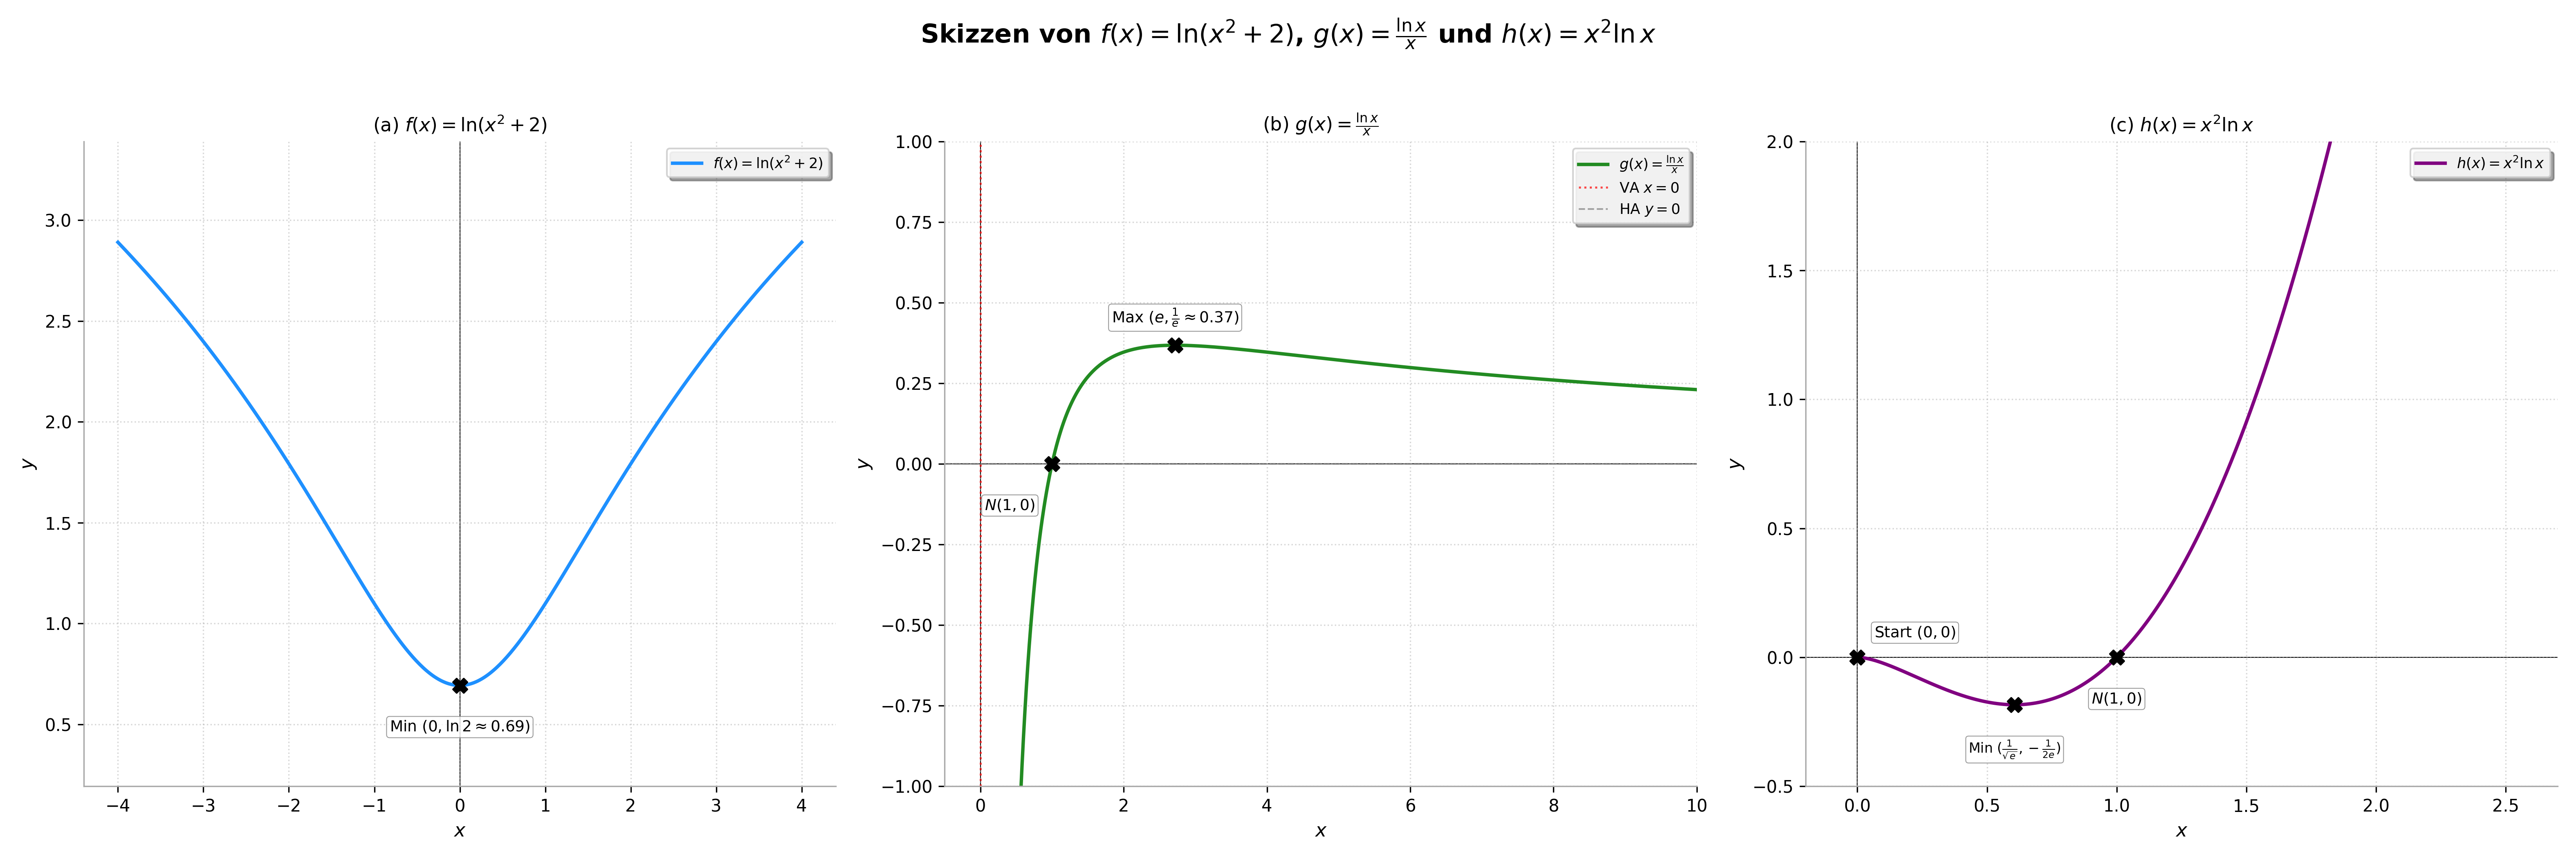
\includegraphics[width=1\textwidth]{grafiken/kurvendiskussion_ln_kombiniert.png}
% --- Beschreibung der Skizze ---
% Die Skizze sollte versuchen, die drei Graphen darzustellen, ggf. mit unterschiedlichen y-Achsen oder in separaten Panels innerhalb einer Abbildung.
% f(x) = ln(x^2+2): Symmetrische Kurve, Min(0, ln2), keine Nst.
% g(x) = ln(x)/x: Für x>0, Asymptote x=0 (nach -unendlich), Nst(1,0), Max(e, 1/e), Asymptote y=0 (nach +unendlich).
% h(x) = x^2 ln(x): Für x>0, startet bei (0,0), Nst(1,0), Min(1/sqrt(e), -1/(2e)), geht nach +unendlich.
% Die Darstellung aller drei in einem sinnvollen gemeinsamen Maßstab ist herausfordernd.
\captionof{figure}{Skizze der Graphen von $f(x)=\ln(x^2+2)$, $g(x)=\frac{\ln x}{x}$ und $h(x)=x^2\ln x$ (konzeptionell).}
\label{fig:kurvendiskussion_ln_kombiniert}
\end{center}

\end{loesungsumgebung}



\begin{aufgabenumgebung}{Integration mit Logarithmusfunktionen üben}
\begin{enumerate}
    \item Berechne die folgenden unbestimmten Integrale:
        \begin{itemize}
            \item $\int (3\ln(x) - 2x) \,dx$
            \item $\int \frac{5x^4}{x^5+1} \,dx$
            \item $\int \frac{e^x}{e^x+3} \,dx$
            \item $\int \frac{1}{2x+7} \,dx$ (Tipp: Erweitere so, dass der Zähler die Ableitung des Nenners ist.)
        \end{itemize}
    \item \textbf{Flächenberechnung:}
        Die Funktion $f(x) = \frac{1}{x}$ ist im ersten Quadranten gegeben.
        \begin{itemize}
            \item Berechne den Inhalt der Fläche, die der Graph von $f(x)$ mit der x-Achse im Intervall $[1, e]$ einschließt.
            \item Berechne den Inhalt der Fläche, die der Graph von $f(x)$ mit der x-Achse im Intervall $[1, b]$ für ein beliebiges $b>1$ einschließt. Was passiert mit dieser Fläche, wenn $b \to \infty$? (Uneigentliches Integral)
        \end{itemize}
    \item \textbf{Anwendung partielle Integration (anspruchsvoller):}
        Berechne $\int x^2 \ln(x) \,dx$. (Tipp: Wähle $v(x)=\ln(x)$ und $u'(x)=x^2$).
\end{enumerate}
\end{aufgabenumgebung}



\begin{loesungsumgebung}[loes:integration-ln-funktionen-ueben]{Integration mit Logarithmusfunktionen üben}

\begin{enumerate}[label=(\alph*)]
    \item \textbf{Berechne die folgenden unbestimmten Integrale:}
    \begin{itemize}
        \item $\mathbf{\int (3\ln(x) - 2x) \,dx}$ \\
        Für diesen Integranden muss $x>0$ sein, damit $\ln(x)$ definiert ist.
        Wir verwenden $\int \ln(x) \,dx = x\ln(x) - x + C_0$ (herleitbar durch partielle Integration).
        \begin{align*} \int (3\ln(x) - 2x) \,dx &= 3\int \ln(x) \,dx - 2\int x \,dx \\ &= 3(x\ln(x) - x) - 2\frac{x^2}{2} + C \\ &= \mathbf{3x\ln(x) - 3x - x^2 + C} \end{align*}

        \item $\mathbf{\int \frac{5x^4}{x^5+1} \,dx}$ \\
        Dieser Integrand ist von der Form $k \cdot \frac{u'(x)}{u(x)}$.
        Sei $u = x^5+1$. Dann ist $\frac{du}{dx} = 5x^4$, also $du = 5x^4 \,dx$.
        \begin{align*} \int \frac{5x^4}{x^5+1} \,dx &= \int \frac{1}{x^5+1} \cdot (5x^4 \,dx) \\ &= \int \frac{1}{u} \,du \\ &= \ln|u| + C \end{align*}
        Rücksubstitution $u=x^5+1$:
        $$ \mathbf{\ln|x^5+1| + C} $$

        \item $\mathbf{\int \frac{e^x}{e^x+3} \,dx}$ \\
        Sei $u = e^x+3$. Dann ist $\frac{du}{dx} = e^x$, also $du = e^x \,dx$.
        \begin{align*} \int \frac{e^x}{e^x+3} \,dx &= \int \frac{1}{e^x+3} \cdot (e^x \,dx) \\ &= \int \frac{1}{u} \,du \\ &= \ln|u| + C \end{align*}
        Rücksubstitution $u=e^x+3$. Da $e^x > 0$ für alle $x$, ist $e^x+3 > 3$ und somit immer positiv. Der Betrag kann entfallen.
        $$ \mathbf{\ln(e^x+3) + C} $$

        \item $\mathbf{\int \frac{1}{2x+7} \,dx}$ \\
        Sei $u = 2x+7$. Dann ist $\frac{du}{dx} = 2$, also $du = 2 \,dx \Rightarrow dx = \frac{1}{2} \,du$.
        \begin{align*} \int \frac{1}{2x+7} \,dx &= \int \frac{1}{u} \cdot \frac{1}{2} \,du \\ &= \frac{1}{2} \int \frac{1}{u} \,du \\ &= \frac{1}{2}\ln|u| + C \end{align*}
        Rücksubstitution $u=2x+7$:
        $$ \mathbf{\frac{1}{2}\ln|2x+7| + C} $$
    \end{itemize}

    \item \textbf{Flächenberechnung mit $f(x) = \frac{1}{x}$ im ersten Quadranten:}
    Im ersten Quadranten ist $x>0$, somit ist $f(x)=\frac{1}{x} > 0$. Die Stammfunktion ist $\ln(x)$.
    \begin{itemize}
        \item \textbf{Flächeninhalt im Intervall $[1, e]$:}
        $$ A_1 = \int_1^e \frac{1}{x} \,dx = [\ln(x)]_1^e = \ln(e) - \ln(1) = 1 - 0 = \mathbf{1} $$
        Der Flächeninhalt beträgt $1$ Flächeneinheit.

        \item \textbf{Flächeninhalt im Intervall $[1, b]$ für $b>1$ und Grenzwert für $b \to \infty$:}
        $$ A_b = \int_1^b \frac{1}{x} \,dx = [\ln(x)]_1^b = \ln(b) - \ln(1) = \ln(b) - 0 = \mathbf{\ln(b)} $$
        Für $b \to \infty$:
        $$ \lim_{b \to \infty} A_b = \lim_{b \to \infty} \ln(b) = \mathbf{\infty} $$
        Die Fläche unter dem Graphen von $f(x)=\frac{1}{x}$ ab $x=1$ bis ins Unendliche ist unendlich groß (das uneigentliche Integral divergiert).
    \end{itemize}

    \item \textbf{Anwendung partielle Integration (anspruchsvoller): $\int x^2 \ln(x) \,dx$} \\
    Für $\ln(x)$ muss $x>0$ sein. Wir wählen (gemäß Tipp, $v(x)$ wird abgeleitet, $u'(x)$ wird integriert, was der Standardwahl $f(x)=\ln(x)$ und $g'(x)=x^2$ entspricht):
    \begin{itemize}
        \item $f(x) = \ln(x) \Rightarrow f'(x) = \frac{1}{x}$
        \item $g'(x) = x^2 \Rightarrow g(x) = \frac{x^3}{3}$
    \end{itemize}
    Anwendung der Formel $\int f(x)g'(x) \,dx = f(x)g(x) - \int f'(x)g(x) \,dx$:
    \begin{align*} \int x^2 \ln(x) \,dx &= \ln(x) \cdot \frac{x^3}{3} - \int \frac{1}{x} \cdot \frac{x^3}{3} \,dx \\ &= \frac{x^3}{3}\ln(x) - \int \frac{x^2}{3} \,dx \\ &= \frac{x^3}{3}\ln(x) - \frac{1}{3} \int x^2 \,dx \\ &= \frac{x^3}{3}\ln(x) - \frac{1}{3} \cdot \frac{x^3}{3} + C \\ &= \mathbf{\frac{x^3}{3}\ln(x) - \frac{x^3}{9} + C} \quad \text{oder} \quad \mathbf{\frac{x^3}{9}(3\ln(x) - 1) + C} \end{align*}
\end{enumerate}

\end{loesungsumgebung}








\begin{aufgabenumgebung}{Checkliste: Das Wesen des Logarithmus und der $\ln$-Funktion verstehen}
Der Logarithmus, insbesondere der natürliche Logarithmus $\ln(x)$, ist ein Schlüsselkonzept mit vielen Facetten. Diese Fragen helfen dir, die Grundlagen zu festigen:

\begin{enumerate}[label=(\alph*)]
    \item \textbf{Definition und Umkehrbeziehung:}
    \begin{itemize}
        \item Erkläre mit eigenen Worten, was $\log_b(y)=x$ bedeutet. Was ist die spezielle Basis beim natürlichen Logarithmus $\ln(x)$?
        \item Warum muss gelten: $e^{\ln(x)} = x$ (für $x>0$) und $\ln(e^x) = x$ (für alle $x \in \mathbb{R}$)? Erläutere dies am Konzept der Umkehrfunktion.
        \item Begründe, warum $\ln(1)=0$ und $\ln(e)=1$ sein muss.
    \end{itemize}
    \item \textbf{Definitionsbereich und Graph:}
    \begin{itemize}
        \item Warum ist der Definitionsbereich der Funktion $f(x)=\ln(x)$ auf positive reelle Zahlen ($x>0$) beschränkt? Wie hängt das mit dem Wertebereich der $e$-Funktion zusammen?
        \item Beschreibe die wesentlichen Unterschiede im Graphenverlauf zwischen $g(x)=e^x$ und $f(x)=\ln(x)$ bezüglich Monotonie, Krümmung und Asymptoten. Wie kommt die geometrische Beziehung (Spiegelung an $y=x$) zustande?
    \end{itemize}
    \item \textbf{Logarithmengesetze anwenden und verstehen:}
    \begin{itemize}
        \item Die Regel $\ln(u^r) = r \cdot \ln(u)$ ist besonders nützlich beim Lösen von Exponentialgleichungen. Erkläre, warum diese Regel das 'Herunterholen' des Exponenten ermöglicht.
        \item Ist die Aussage $\ln(a+b) = \ln(a) + \ln(b)$ korrekt? Überprüfe mit einem Zahlenbeispiel und vergleiche mit der Produktregel $\ln(a \cdot b) = \ln(a) + \ln(b)$.
    \end{itemize}
\end{enumerate}
\end{aufgabenumgebung}

\begin{loesungsumgebung}[loes:checkliste-logarithmus-ln-verstehen]{Checkliste: Das Wesen des Logarithmus und der $\ln$-Funktion verstehen}

\begin{enumerate}[label=(\alph*)]
    \item \textbf{Definition und Umkehrbeziehung:}
    \begin{itemize}
        \item \textbf{Bedeutung von $\log_b(y)=x$ und die Basis des natürlichen Logarithmus:} \\
        Die Gleichung $\log_b(y)=x$ ist die logarithmische Schreibweise für die Exponentialgleichung $b^x = y$. Sie bedeutet: 'Der Logarithmus von $y$ zur Basis $b$ ist der Exponent $x$, mit dem die Basis $b$ potenziert werden muss, um $y$ zu erhalten.' Dabei muss die Basis $b$ positiv und ungleich 1 sein ($b>0, b \neq 1$), und das Argument des Logarithmus $y$ muss positiv sein ($y>0$).
        Der \textbf{natürliche Logarithmus}, geschrieben als $\ln(x)$, hat als spezielle Basis die \textbf{Eulersche Zahl $e \approx 2.71828$}. Es gilt also: $\ln(x) = \log_e(x)$.

        \item \textbf{Warum $e^{\ln(x)} = x$ (für $x>0$) und $\ln(e^x) = x$ (für alle $x \in \mathbb{R}$)?} \\
        Dies ergibt sich direkt aus der Definition des Logarithmus als Umkehrfunktion zur Exponentialfunktion.
        \begin{itemize}
            \item $f(x)=e^x$ und $g(x)=\ln(x)$ sind Umkehrfunktionen zueinander.
            \item Für Umkehrfunktionen gilt allgemein: $f(g(x))=x$ für $x$ im Definitionsbereich von $g$, und $g(f(x))=x$ für $x$ im Definitionsbereich von $f$.
            \item $e^{\ln(x)} = x$: Hier wird $\ln(x)$ (der Exponent, mit dem $e$ potenziert $x$ ergibt) wieder als Exponent von $e$ verwendet. Das Ergebnis muss $x$ sein. Dies gilt für $x>0$, da $\ln(x)$ nur für positive $x$ definiert ist.
            \item $\ln(e^x) = x$: Hier wird der Logarithmus von $e^x$ gebildet. Die Frage ist: 'Mit welcher Zahl muss $e$ potenziert werden, um $e^x$ zu erhalten?' Die Antwort ist $x$. Dies gilt für alle reellen Zahlen $x$, da $e^x$ immer positiv und somit im Definitionsbereich des Logarithmus ist.
        \end{itemize}

        \item \textbf{Begründung für $\ln(1)=0$ und $\ln(e)=1$:}
        \begin{itemize}
            \item $\ln(1)=0$: Wir suchen die Zahl $x$, für die $e^x=1$ gilt. Da jede Zahl (außer 0) hoch 0 gleich 1 ist, also $e^0=1$, muss $\ln(1)=0$ sein.
            \item $\ln(e)=1$: Wir suchen die Zahl $x$, für die $e^x=e$ gilt. Dies ist offensichtlich $x=1$, da $e^1=e$. Also muss $\ln(e)=1$ sein.
        \end{itemize}
    \end{itemize}

    \item \textbf{Definitionsbereich und Graph:}
    \begin{itemize}
        \item \textbf{Warum ist der Definitionsbereich von $f(x)=\ln(x)$ auf $x>0$ beschränkt?} \\
        Der Logarithmus $\ln(x)=y$ ist definiert als die Umkehrung von $e^y=x$. Die Exponentialfunktion $e^y$ nimmt für alle reellen Exponenten $y$ ausschließlich positive Werte an (der Wertebereich von $e^y$ ist $(0, \infty)$). Da $x$ das Ergebnis von $e^y$ ist, muss $x$ zwingend positiv sein. Es gibt keine reelle Zahl $y$, für die $e^y$ Null oder negativ wäre.
        Daher ist der Definitionsbereich der natürlichen Logarithmusfunktion die Menge der positiven reellen Zahlen, $D_f = (0, \infty)$.

        \item \textbf{Unterschiede im Graphenverlauf zwischen $g(x)=e^x$ und $f(x)=\ln(x)$:}
        \begin{itemize}
            \item \textbf{Monotonie:} Beide Funktionen sind streng monoton steigend in ihrem gesamten Definitionsbereich.
            \item \textbf{Krümmung:}
            $g(x)=e^x$: $g''(x)=e^x > 0$ für alle $x$. Der Graph ist immer linksgekrümmt (konvex).
            $f(x)=\ln(x)$: $f''(x)=-1/x^2 < 0$ für $x>0$. Der Graph ist immer rechtsgekrümmt (konkav).
            \item \textbf{Asymptoten:}
            $g(x)=e^x$: Hat eine horizontale Asymptote $y=0$ für $x \to -\infty$. Keine senkrechten Asymptoten.
            $f(x)=\ln(x)$: Hat eine senkrechte Asymptote $x=0$ (die y-Achse) für $x \to 0^+$, wobei $f(x) \to -\infty$. Keine horizontalen Asymptoten ($f(x) \to \infty$ für $x \to \infty$).
            \item \textbf{Achsenschnittpunkte:}
            $g(x)=e^x$: y-Achsenabschnitt $(0|1)$, keine Nullstellen.
            $f(x)=\ln(x)$: x-Achsenabschnitt (Nullstelle) $(1|0)$, keinen y-Achsenabschnitt.
            \item \textbf{Definitions-/Wertebereich:}
            $g(x)=e^x$: $D_g=\mathbb{R}$, $W_g=(0, \infty)$.
            $f(x)=\ln(x)$: $D_f=(0, \infty)$, $W_f=\mathbb{R}$. (Definitions- und Wertebereich sind vertauscht).
        \end{itemize}
        \textbf{Geometrische Beziehung:} Da $f(x)=\ln(x)$ die Umkehrfunktion von $g(x)=e^x$ ist, gehen ihre Graphen durch \textbf{Spiegelung an der Geraden $y=x$} (der Winkelhalbierenden des I. und III. Quadranten) auseinander hervor.
    \end{itemize}

    \item \textbf{Logarithmengesetze anwenden und verstehen:}
    \begin{itemize}
        \item \textbf{Regel $\ln(u^r) = r \cdot \ln(u)$ und das 'Herunterholen' des Exponenten:}
        Diese Regel besagt, dass der Logarithmus einer Potenz gleich dem Exponenten multipliziert mit dem Logarithmus der Basis dieser Potenz ist.
        Beim Lösen von Exponentialgleichungen der Form $b^x=y$ ist diese Regel zentral:
        1. Man logarithmiert beide Seiten der Gleichung: $\ln(b^x) = \ln(y)$.
        2. Mit der Regel $\ln(u^r) = r \cdot \ln(u)$ kann man den Exponenten $x$ als Faktor vor den Logarithmus ziehen: $x \cdot \ln(b) = \ln(y)$.
        3. Nun kann man nach $x$ auflösen: $x = \frac{\ln(y)}{\ln(b)}$.
        Die Regel ermöglicht es also, den Exponenten $x$ aus der Potenz 'herauszuholen' und ihn so einer direkten Berechnung zugänglich zu machen.

        \item \textbf{Ist die Aussage $\ln(a+b) = \ln(a) + \ln(b)$ korrekt?}
        Die Aussage $\ln(a+b) = \ln(a) + \ln(b)$ ist \textbf{falsch}.
        \textit{Zahlenbeispiel:} Seien $a=1$ und $b=e-1$ (beide positiv).
        $\ln(a+b) = \ln(1 + e-1) = \ln(e) = 1$.
        $\ln(a) + \ln(b) = \ln(1) + \ln(e-1) = 0 + \ln(e-1)$.
        Da $e-1 \approx 1.718$, ist $\ln(e-1) \approx \ln(1.718) \approx 0.541$.
        Somit ist $1 \neq 0.541$.
        \textit{Vergleich mit der Produktregel:} Die korrekte Regel für die Summe von Logarithmen ist das Logarithmus eines Produkts: $\mathbf{\ln(a \cdot b) = \ln(a) + \ln(b)}$. Für den Logarithmus einer Summe ($\ln(a+b)$) gibt es keine vergleichbare einfache Zerlegungsregel.
    \end{itemize}
\end{enumerate}

\end{loesungsumgebung}





\begin{aufgabenumgebung}{Checkliste: Analysis mit der $\ln$-Funktion – Ableiten, Integrieren, Anwenden}
Die $\ln$-Funktion und ihre Ableitung $1/x$ tauchen in vielen analytischen Zusammenhängen auf.

\begin{enumerate}[label=(\alph*)]
    \item \textbf{Ableiten mit $\ln(x)$:}
    \begin{itemize}
        \item Die Ableitung von $\ln(x)$ ist $1/x$. Was sagt dir das über die Steigung des Graphen von $\ln(x)$ für $x$-Werte nahe Null (aber $x>0$) im Vergleich zu sehr großen $x$-Werten?
        \item Bei der Ableitung von $\ln(h(x))$ lautet die Regel $\frac{h'(x)}{h(x)}$. Erkläre, wie die Kettenregel hier zur Anwendung kommt ($g(u)=\ln u \implies g'(u)=1/u$).
    \end{itemize}
    \item \textbf{Integrieren mit $\ln(x)$:}
    \begin{itemize}
        \item Warum schreiben wir $\int \frac{1}{x} \,dx = \ln|x|+C$ mit Betragsstrichen, obwohl der Definitionsbereich von $\ln(x)$ selbst $x>0$ ist?
        \item Für die Berechnung von $\int \ln(x) \,dx$ wurde die partielle Integration mit $u'(x)=1$ und $v(x)=\ln(x)$ genutzt. Warum wäre die Wahl $u'(x)=\ln(x)$ und $v(x)=1$ nicht zielführend, wenn du $\int \ln(x) \,dx$ noch nicht kennst?
        \item Erkläre, warum das Integral $\int \frac{g'(x)}{g(x)} \,dx$ auf $\ln|g(x)|+C$ führt. Welche Substitution steckt dahinter?
    \end{itemize}
    \item \textbf{Kurvendiskussion und Grenzwerte:}
    \begin{itemize}
        \item Wenn du eine Funktion wie $f(x)=x^2 \ln(x)$ untersuchst: Welcher der beiden Faktoren ($x^2$ oder $\ln(x)$) 'dominiert' das Verhalten für $x \to \infty$? Und für $x \to 0^+$? (Denke an die bekannten Grenzwerte $\lim_{x \to \infty} \frac{\ln x}{x^n}=0$ und $\lim_{x \to 0^+} x^n \ln x = 0$).
        \item Welche Schritte sind bei einer Kurvendiskussion einer Funktion mit $\ln(x)$ besonders wichtig im Hinblick auf den Definitionsbereich?
    \end{itemize}
\end{enumerate}
\end{aufgabenumgebung}

\begin{loesungsumgebung}[loes:checkliste-ln-funktion-analysis]{Checkliste: Analysis mit der $\ln$-Funktion – Ableiten, Integrieren, Anwenden}

\begin{enumerate}[label=(\alph*)]
    \item \textbf{Ableiten mit $\ln(x)$:}
    \begin{itemize}
        \item \textbf{Ableitung von $\ln(x)$ und Steigung des Graphen:} \\
        Die Ableitung von $f(x)=\ln(x)$ ist $f'(x)=\frac{1}{x}$.
        \begin{itemize}
            \item Für $x$-Werte nahe Null (aber $x>0$, z.B. $x=0.01$): $f'(x) = \frac{1}{x}$ wird sehr groß (z.B. $1/0.01 = 100$). Das bedeutet, der Graph von $\ln(x)$ ist für $x$-Werte nahe Null (von rechts kommend) \textbf{sehr steil ansteigend} (obwohl die Funktionswerte $f(x)$ gegen $-\infty$ gehen).
            \item Für sehr große $x$-Werte (z.B. $x=100$): $f'(x) = \frac{1}{x}$ wird sehr klein (z.B. $1/100 = 0.01$). Das bedeutet, der Graph von $\ln(x)$ wird für große $x$-Werte \textbf{immer flacher}, obwohl er weiterhin streng monoton steigt.
        \end{itemize}

        \item \textbf{Ableitung von $\ln(h(x))$ mit der Kettenregel:} \\
        Sei $f(x) = \ln(h(x))$. Wir wenden die Kettenregel $(a(i(x)))' = a'(i(x)) \cdot i'(x)$ an.
        Die äußere Funktion ist $a(u) = \ln(u)$, deren Ableitung $a'(u) = \frac{1}{u}$ ist.
        Die innere Funktion ist $i(x) = h(x)$, deren Ableitung $i'(x) = h'(x)$ ist.
        Somit ist die Ableitung von $f(x) = \ln(h(x))$:
        $$ f'(x) = a'(h(x)) \cdot h'(x) = \frac{1}{h(x)} \cdot h'(x) = \mathbf{\frac{h'(x)}{h(x)}} $$
    \end{itemize}

    \item \textbf{Integrieren mit $\ln(x)$:}
    \begin{itemize}
        \item \textbf{Warum $\int \frac{1}{x} \,dx = \ln|x|+C$ mit Betragsstrichen?} \\
        Die Funktion $f(x)=\frac{1}{x}$ ist für alle $x \neq 0$ definiert. Ihre Stammfunktion muss also ebenfalls für alle $x \neq 0$ definiert sein (bzw. auf getrennten Intervallen $(-\infty,0)$ und $(0,\infty)$).
        \begin{itemize}
            \item Für $x>0$: $(\ln(x))' = \frac{1}{x}$. Also ist $\ln(x)$ eine Stammfunktion für $x>0$.
            \item Für $x<0$: Sei $y=-x$. Dann ist $y>0$. Die Ableitung von $\ln(-x)$ ist nach der Kettenregel: $(\ln(-x))' = \frac{1}{-x} \cdot (-1) = \frac{1}{x}$. Also ist $\ln(-x)$ eine Stammfunktion für $x<0$.
        \end{itemize}
        Beide Fälle können zusammengefasst werden als $(\ln|x|)' = \frac{1}{x}$ für $x \neq 0$. Die Betragsstriche stellen sicher, dass das Argument des Logarithmus positiv ist und der Definitionsbereich der Stammfunktion (bis auf $x=0$) dem von $\frac{1}{x}$ entspricht. Daher ist die allgemeinste Stammfunktion $\ln|x|+C$.

        \item \textbf{Partielle Integration von $\int \ln(x) \,dx$:} \\
        Für $\int \ln(x) \,dx = \int 1 \cdot \ln(x) \,dx$ wählt man typischerweise:
        $u'(x)=1 \Rightarrow u(x)=x$
        $v(x)=\ln(x) \Rightarrow v'(x)=\frac{1}{x}$
        Dies führt zu: $\int \ln(x) \,dx = x\ln(x) - \int x \cdot \frac{1}{x} \,dx = x\ln(x) - \int 1 \,dx = x\ln(x) - x + C$.
        Die Wahl $u'(x)=\ln(x)$ und $v(x)=1$ wäre nicht zielführend, wenn man $\int \ln(x) \,dx$ noch nicht kennt, weil man dann $u(x) = \int \ln(x) \,dx$ bestimmen müsste, was ja gerade das gesuchte Integral ist. Man würde also die Kenntnis der Lösung voraussetzen:
        $\int \ln(x) \cdot 1 \,dx = (\int \ln(x) \,dx) \cdot 1 - \int (\int \ln(x) \,dx) \cdot 0 \,dx = \int \ln(x) \,dx$. Dies ist eine triviale Gleichung und hilft nicht weiter.

        \item \textbf{Warum $\int \frac{g'(x)}{g(x)} \,dx = \ln|g(x)|+C$?} \\
        Dies ergibt sich direkt aus der Substitutionsregel (Umkehrung der Kettenregel).
        Wir wählen die Substitution $u = g(x)$.
        Dann ist das Differential $\frac{du}{dx} = g'(x)$, also $du = g'(x) \,dx$.
        Das Integral transformiert sich damit zu:
        $$ \int \frac{g'(x)}{g(x)} \,dx = \int \frac{1}{g(x)} \cdot (g'(x) \,dx) = \int \frac{1}{u} \,du $$
        Die Stammfunktion von $\frac{1}{u}$ ist $\ln|u|$. Setzt man die Konstante $C$ hinzu und substituiert $u=g(x)$ zurück, erhält man:
        $$ \ln|g(x)| + C $$
    \end{itemize}

    \item \textbf{Kurvendiskussion und Grenzwerte:}
    \begin{itemize}
        \item \textbf{Dominanz bei $f(x)=x^2 \ln(x)$ für $x \to \infty$ und $x \to 0^+$:}
        \begin{itemize}
            \item Für $\mathbf{x \to \infty}$: Beide Faktoren $x^2$ und $\ln(x)$ gehen gegen $\infty$. Ihr Produkt $x^2\ln(x)$ geht daher ebenfalls gegen $\mathbf{\infty}$. Obwohl $x^2$ schneller wächst als $\ln(x)$, 'dominieren' hier beide Faktoren das Wachstum gemeinsam ins Unendliche.
            \item Für $\mathbf{x \to 0^+}$: $x^2 \to 0$ und $\ln(x) \to -\infty$. Wir haben einen Ausdruck vom Typ $0 \cdot (-\infty)$, der unbestimmt ist. Der Grenzwert $\lim_{x \to 0^+} x^n \ln x = 0$ (für $n>0$) ist bekannt. Hier ist $n=2$.
            Also $\lim_{x \to 0^+} x^2 \ln(x) = \mathbf{0}$.
            In diesem Fall 'dominiert' der Potenzterm $x^2$ (der gegen Null geht) über den logarithmischen Term $\ln(x)$ (der gegen $-\infty$ geht) und zieht das Produkt gegen Null.
        \end{itemize}

        \item \textbf{Wichtige Schritte bei Kurvendiskussion einer Funktion mit $\ln(x)$ bezüglich Definitionsbereich:}
        \begin{enumerate}
            \item \textbf{Argument des Logarithmus bestimmen:} Identifiziere alle Terme der Form $\ln(h(x))$.
            \item \textbf{Bedingung für das Argument aufstellen:} Für jeden Logarithmusterm muss gelten, dass sein Argument strikt positiv ist: $h(x) > 0$.
            \item \textbf{Ungleichung(en) lösen:} Löse diese Ungleichung(en), um die erlaubten $x$-Werte zu finden. Dies ergibt den Definitionsbereich der Funktion.
            \item \textbf{Verhalten an den Rändern des Definitionsbereichs untersuchen:} Bestimme die Grenzwerte der Funktion, wenn sich $x$ den Rändern des Definitionsbereichs nähert (insbesondere an Stellen, wo das Argument des Logarithmus gegen Null geht, da dies oft zu senkrechten Asymptoten führt, weil $\ln(u) \to -\infty$ für $u \to 0^+$).
            \item \textbf{Definitionsbereich bei Ableitungen beachten:} Die Ableitungen können zusätzliche Einschränkungen im Definitionsbereich haben (z.B. wenn $h(x)$ im Nenner von $f'(x)$ auftaucht), aber der Definitionsbereich der ursprünglichen Funktion $f(x)$ ist maßgeblich für die Analyse von $f(x)$ selbst.
        \end{enumerate}
    \end{itemize}
\end{enumerate}

\end{loesungsumgebung}